\section{Results}\label{sec:literature-review-results}
In this section, we report the key findings of our study.

\subsection{Why are DT and SoS principles combined? (RQ1)}\label{sec:results-rq1}
We address why SoS and DT principles are combined by analyzing the motivations, integration intents, and application domains of SoTS.

\subsubsection{Motivations}\label{sec:motivations}
\begin{table*}[htp]
            \centering
            \scriptsize
            \caption{Motivations for combining DT and SoS}
            \label{tab:motivations-table}
            \begin{tabular}{@{}p{4cm}l p{8.5cm}@{}}
            \toprule
            \multicolumn{1}{c}{\textbf{Motivation}} & 
            \multicolumn{1}{c}{\textbf{Frequency}} & 
            \multicolumn{1}{c}{\textbf{Studies}} \\ 
            \midrule
            Optimization & \maindatabar{30} & \cite{bao2024digital,becue2018cyberfactory,chavezbaliguat2023digital,chen2018digital,duan2023digital,folds2019digital,gill2022method,howard2021greenhouse,jirsa2024use,joseph2021aggregated,kruger2022towards,lee2022simulation,li2022cognitive,li2024comprehensive,lippi2023enabling,liu2020web-based,maheshwari2022digital,malayjerdi2022combined,novak2022digitalized,park2020digital,pickering2023towards,pillai2023digital,potteiger2023live,priyanta2024is,somma2023digital,vermesan2021internet,villalonga2021decision-making,wullink2024foundational,zhang2022multi-scale,zhang2021bi-level} \\
Integration & \maindatabar{25} & \cite{acharya2023twins,alam2017c2ps,ashtaritalkhestani2019architecture,aziz2022empowering,bellavista2023requirements,demir2023vertically-integrated,dobie2024network,doubell2023digital,esterle2021digital,gil2023modeling,gil2024integrating,gollner2022collaborative,hatledal2020co-simulation,heininger2021capturing,heithoff2023challenges,hofmeister2024cross-domain,hofmeister2024semantic,human2023design,larsen2024towards,mahoro2023articulating,monsalve2021novel,reiche2021digital,savur2019hrc-sos,stary2022privacy,vogel-heuser2021approach} \\
Validation & \maindatabar{15} & \cite{bertoni2022digital,clark2021chapter,coupaye2023graph-based,dahmen2022modeling,dickopf2019holistic,ehemann2023digital,kulkarni2019towards,marah2023architecture,mavromatis2024umbrella,oquendo2019dealing,redelinghuys2020six-layer,samak2023autodrive,schluse2017experimentable,wagner2023using,wang2024construction} \\
Maintainability & \maindatabar{10} & \cite{altamiranda2019system,barden2022academic,binder2021utilizing,hatakeyama2018systems,jiang2022novel,kutzke2021subsystem,lopez2023modeling,parri2021framework,parri2019jarvis,saraeian2022digital} \\
\bottomrule
            \end{tabular}
            \end{table*}
As shown in \tabref{tab:motivations-table}, SoTS are primarily motivated by optimization, followed by integration, validation, and maintainability. Optimization is the most prominent motivation, reflecting the use of SoTS to improve system-level awareness and support coordinated decision-making. For example, SoTS are used to coordinate UAV landings on USVs to minimize operation time \cite{li2022cognitive}. Integration is also common, with studies focusing on connecting heterogeneous systems through coordinated DTs. In power systems, SoTS support coordinated operation across distributed grid elements \cite{monsalve2021novel}. Validation appears less frequently and is typically associated with simulation-based testing of complex or safety-critical interactions, such as advanced driver assistance systems \cite{dahmen2022modeling}. Maintainability is addressed in a smaller subset of studies.


\subsubsection{Intents and application domains}\label{sec:intents}
\begin{table*}[]
            \centering
            \footnotesize
            \caption{Intents of combining DT and SoS}
            \label{tab:intents-table}
            \begin{tabular}{@{}p{4cm}l p{8.5cm}@{}}
            \toprule
            \multicolumn{1}{c}{\textbf{Intent}} & 
            \multicolumn{1}{c}{\textbf{Frequency}} & 
            \multicolumn{1}{c}{\textbf{Studies}} \\ 
            \midrule
            Combining DTs into a SoS & \maindatabar{49} & \cite{acharya2023twins,alam2017c2ps,altamiranda2019system,ashtaritalkhestani2019architecture,aziz2022empowering,barden2022academic,becue2018cyberfactory,bellavista2023requirements,bertoni2022digital,chen2018digital,coupaye2023graph-based,dahmen2022modeling,demir2023vertically-integrated,dickopf2019holistic,doubell2023digital,ehemann2023digital,esterle2021digital,gil2023modeling,gil2024integrating,gill2022method,gollner2022collaborative,hatakeyama2018systems,heininger2021capturing,heithoff2023challenges,hofmeister2024cross-domain,hofmeister2024semantic,howard2021greenhouse,human2023design,jiang2022novel,jirsa2024use,joseph2021aggregated,kruger2022towards,kulkarni2019towards,larsen2024towards,li2022cognitive,lippi2023enabling,liu2020web-based,mahoro2023articulating,marah2023architecture,mavromatis2024umbrella,monsalve2021novel,parri2019jarvis,redelinghuys2020six-layer,reiche2021digital,schluse2017experimentable,stary2022privacy,villalonga2021decision-making,vogel-heuser2021approach,wullink2024foundational} \\
Twinning a SoS & \maindatabar{31} & \cite{bao2024digital,binder2021utilizing,chavezbaliguat2023digital,clark2021chapter,dobie2024network,duan2023digital,folds2019digital,hatledal2020co-simulation,kutzke2021subsystem,lee2022simulation,li2024comprehensive,lopez2023modeling,maheshwari2022digital,malayjerdi2022combined,novak2022digitalized,oquendo2019dealing,park2020digital,parri2021framework,pickering2023towards,pillai2023digital,potteiger2023live,priyanta2024is,samak2023autodrive,saraeian2022digital,savur2019hrc-sos,somma2023digital,vermesan2021internet,wagner2023using,wang2024construction,zhang2022multi-scale,zhang2021bi-level} \\
\bottomrule
            \end{tabular}
            \end{table*}
We distinguish between two intents in SoTS: (i) twinning a SoS and (ii) combining DTs into a SoS. As shown in \tabref{tab:intents-table}, combining DTs into a SoS is more common, indicating a preference for integrating multiple DTs rather than representing a system with a single twin.

\begin{figure}[t]
    \centering
    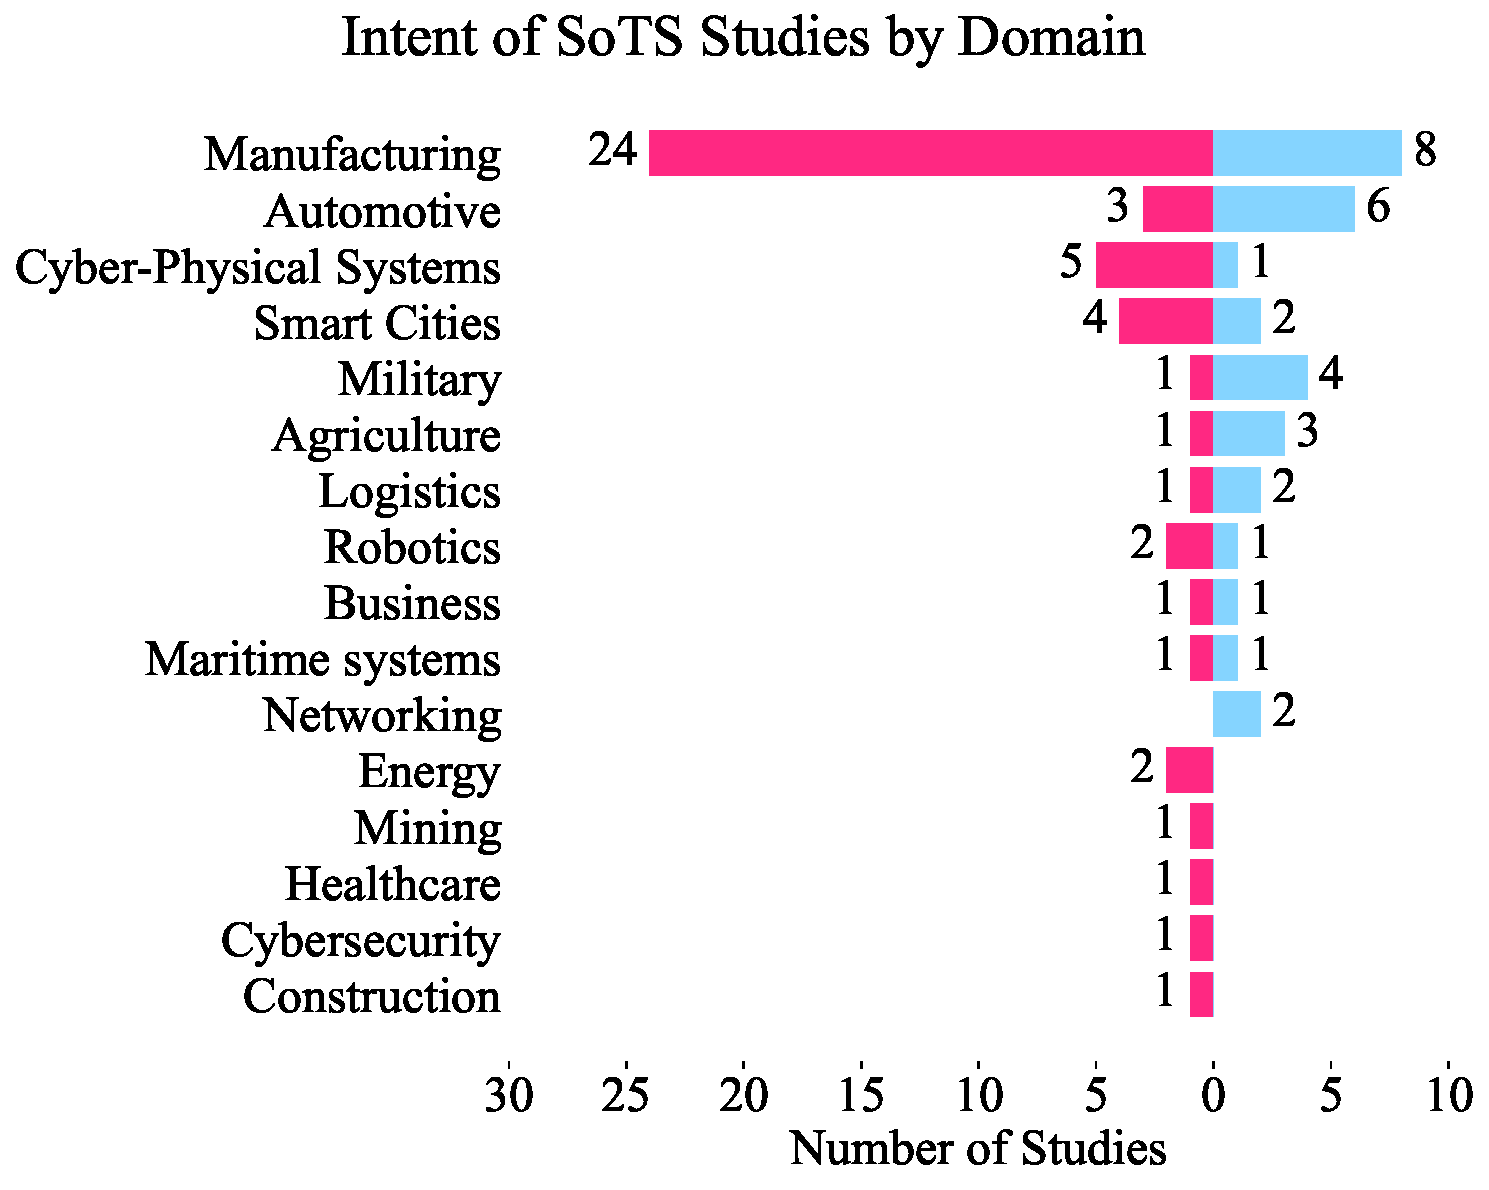
\includegraphics[width=0.65\linewidth]{figures/Literature Review/rq1/intentOfSoSDT.pdf}
    \caption{Intent of SoTS vs Domain}
    \caption*{{\color[HTML]{FF2882}\ding{110}} Combining DTs into a SoS~~~{\color[HTML]{85d4ff}\ding{110}} Twinning a SoS }
    \label{fig:sos-dt-intent}
\end{figure}

\figref{fig:sos-dt-intent} shows how these intents vary across domains. Manufacturing dominates both approaches, with SoTS used to coordinate machines and production lines \cite{villalonga2021decision-making, novak2022digitalized}. Smart cities more often adopt DT combination to coordinate distributed infrastructure, while automotive and military systems more often rely on SoS twinning to support global system awareness. Some domains appear exclusively under one approach. Networking is only observed under SoS twinning, focusing on holistic system oversight \cite{dobie2024network, priyanta2024is}, whereas domains such as energy, mining, healthcare, cybersecurity, and construction appear only under DT combination. Other domains, including smart cities and logistics, use both approaches.

\begin{table*}[]
            \centering
            \footnotesize
            \caption{Application domains}
            \label{tab:domains-table}
            \begin{tabular}{@{}p{4cm}l p{8.5cm}@{}}
            \toprule
            \multicolumn{1}{c}{\textbf{Domain}} & 
            \multicolumn{1}{c}{\textbf{Frequency}} & 
            \multicolumn{1}{c}{\textbf{Studies}} \\ 
            \midrule
            Manufacturing & \maindatabar{32} & \cite{acharya2023twins,ashtaritalkhestani2019architecture,aziz2022empowering,bao2024digital,barden2022academic,bellavista2023requirements,binder2021utilizing,demir2023vertically-integrated,duan2023digital,ehemann2023digital,esterle2021digital,gill2022method,gollner2022collaborative,jirsa2024use,joseph2021aggregated,kruger2022towards,kutzke2021subsystem,larsen2024towards,lippi2023enabling,liu2020web-based,marah2023architecture,monsalve2021novel,novak2022digitalized,park2020digital,parri2019jarvis,redelinghuys2020six-layer,reiche2021digital,schluse2017experimentable,villalonga2021decision-making,vogel-heuser2021approach,zhang2021bi-level,zhang2022multi-scale} \\
Automotive & \maindatabar{9} & \cite{chen2018digital,dahmen2022modeling,heithoff2023challenges,malayjerdi2022combined,oquendo2019dealing,pillai2023digital,potteiger2023live,samak2023autodrive,vermesan2021internet} \\
Cyber-Physical Systems & \maindatabar{6} & \cite{alam2017c2ps,coupaye2023graph-based,li2022cognitive,mahoro2023articulating,parri2021framework,stary2022privacy} \\
Smart Cities & \maindatabar{6} & \cite{hofmeister2024cross-domain,hofmeister2024semantic,human2023design,li2024comprehensive,mavromatis2024umbrella,somma2023digital} \\
Military & \maindatabar{5} & \cite{folds2019digital,hatakeyama2018systems,lee2022simulation,lopez2023modeling,wang2024construction} \\
Agriculture & \maindatabar{4} & \cite{chavezbaliguat2023digital,howard2021greenhouse,pickering2023towards,saraeian2022digital} \\
Logistics & \maindatabar{3} & \cite{clark2021chapter,doubell2023digital,wagner2023using} \\
Robotics & \maindatabar{3} & \cite{gil2023modeling,gil2024integrating,savur2019hrc-sos} \\
Other & \maindatabar{12} & \cite{altamiranda2019system,becue2018cyberfactory,bertoni2022digital,dickopf2019holistic,dobie2024network,hatledal2020co-simulation,heininger2021capturing,jiang2022novel,kulkarni2019towards,maheshwari2022digital,priyanta2024is,wullink2024foundational} \\
\bottomrule
            \end{tabular}
            \end{table*}
As shown in \tabref{tab:domains-table}, manufacturing is the most frequent application domain, followed by automotive and smart cities. The cyber-physical systems domain also appears frequently, focusing on real-time interaction between distributed physical and digital components \cite{alam2017c2ps, stary2022privacy}. Other domains, such as military, agriculture, logistics, and robotics, appear less frequently.

\begin{conclusionframe}{RQ1: Why are DT and SoS combined}
SoTS are developed to support optimization, integration, validation, and maintainability in complex systems. Manufacturing is the most common application domain, followed by automotive and smart cities.
\end{conclusionframe}

\subsection{How are DT and SoS combined? (RQ2)}\label{results-rq2}
To understand how DT and SoS are combined, we analyze architectures and types of constituent units represented in SoTS.

\subsubsection{Architecture Configurations}\label{sec:literature-review-architecture}
\begin{table*}[htp]
            \centering
            \scriptsize
            \caption{SoTS Type}
            \label{tab:sots-type-table}
            \begin{tabular}{@{}p{4cm}l p{8.5cm}@{}}
            \toprule
            \multicolumn{1}{c}{\textbf{SoTS}} & 
            \multicolumn{1}{c}{\textbf{Frequency}} & 
            \multicolumn{1}{c}{\textbf{Studies}} \\ 
            \midrule
            Acknowledged SoTS & \maindatabar{31} & \cite{altamiranda2019system,becue2018cyberfactory,bellavista2023requirements,bertoni2022digital,binder2021utilizing,coupaye2023graph-based,demir2023vertically-integrated,ehemann2023digital,folds2019digital,gill2022method,heininger2021capturing,heithoff2023challenges,human2023design,kruger2022towards,li2022cognitive,lippi2023enabling,lopez2023modeling,maheshwari2022digital,mahoro2023articulating,malayjerdi2022combined,monsalve2021novel,parri2019jarvis,pillai2023digital,potteiger2023live,priyanta2024is,redelinghuys2020six-layer,samak2023autodrive,saraeian2022digital,somma2023digital,wagner2023using,zhang2021bi-level} \\
Directed SoTS & \maindatabar{26} & \cite{alam2017c2ps,ashtaritalkhestani2019architecture,aziz2022empowering,chavezbaliguat2023digital,dickopf2019holistic,dobie2024network,doubell2023digital,duan2023digital,gil2024integrating,hatakeyama2018systems,hofmeister2024semantic,jiang2022novel,kulkarni2019towards,kutzke2021subsystem,larsen2024towards,lee2022simulation,li2024comprehensive,novak2022digitalized,park2020digital,parri2021framework,reiche2021digital,schluse2017experimentable,stary2022privacy,villalonga2021decision-making,wang2024construction,zhang2022multi-scale} \\
Collaborative SoTS & \maindatabar{19} & \cite{acharya2023twins,bao2024digital,barden2022academic,chen2018digital,dahmen2022modeling,gil2023modeling,gollner2022collaborative,hatledal2020co-simulation,hofmeister2024cross-domain,howard2021greenhouse,jirsa2024use,joseph2021aggregated,liu2020web-based,marah2023architecture,mavromatis2024umbrella,savur2019hrc-sos,vermesan2021internet,vogel-heuser2021approach,wullink2024foundational} \\
Virtual SoTS & \maindatabar{4} & \cite{clark2021chapter,esterle2021digital,oquendo2019dealing,pickering2023towards} \\
\bottomrule
            \end{tabular}
            \end{table*}
The distribution of SoTS architectures, based on the classification framework defined in \secref{sec:literature-review-classification}, is shown in \tabref{tab:sots-type-table}. Acknowledged and directed SoTS are the most common configurations. In acknowledged SoTS, a central DT facilitates coordination while constituents retain managerial independence and negotiate their own goals. For example, \textcite{li2022cognitive} use a cognitive twin to provide recommendations while constituent systems retain control, and \textcite{monsalve2021novel} use a DT Master to coordinate grid simulations. Directed SoTS include a central DT that orchestrates constituent behavior, as seen in systems where a DT aggregates and controls machine-level twins \cite{reiche2021digital, li2024comprehensive}.

Collaborative SoTS appear less frequently and rely on decentralized coordination among DTs, where coordination occurs through local interaction and negotiation, such as in decentralized manufacturing or connected vehicle systems \cite{vogel-heuser2021approach, chen2018digital}. Virtual SoTS are rare and involve loosely coupled systems that coordinate dynamically without predefined control structures.


\subsubsection{Constituent units}\label{sec:constituents}
\begin{table*}[]
            \centering
            \footnotesize
            \caption{Constituent units}
            \label{tab:constituent-units-table}
            \begin{tabular}{@{}p{4cm}l p{8.5cm}@{}}
            \toprule
            \multicolumn{1}{c}{\textbf{Constituent Unit}} & 
            \multicolumn{1}{c}{\textbf{Frequency}} & 
            \multicolumn{1}{c}{\textbf{Studies}} \\ 
            \midrule
            Physical Systems & \maindatabar{62} & \cite{acharya2023twins,altamiranda2019system,ashtaritalkhestani2019architecture,aziz2022empowering,bao2024digital,barden2022academic,becue2018cyberfactory,bellavista2023requirements,bertoni2022digital,binder2021utilizing,chavezbaliguat2023digital,chen2018digital,coupaye2023graph-based,dahmen2022modeling,demir2023vertically-integrated,dobie2024network,doubell2023digital,duan2023digital,ehemann2023digital,esterle2021digital,gil2023modeling,gill2022method,gollner2022collaborative,hatledal2020co-simulation,heininger2021capturing,heithoff2023challenges,hofmeister2024cross-domain,hofmeister2024semantic,howard2021greenhouse,human2023design,jiang2022novel,jirsa2024use,joseph2021aggregated,kruger2022towards,kutzke2021subsystem,larsen2024towards,lee2022simulation,li2022cognitive,li2024comprehensive,lippi2023enabling,liu2020web-based,lopez2023modeling,malayjerdi2022combined,monsalve2021novel,novak2022digitalized,oquendo2019dealing,park2020digital,pillai2023digital,potteiger2023live,redelinghuys2020six-layer,reiche2021digital,samak2023autodrive,saraeian2022digital,somma2023digital,vermesan2021internet,villalonga2021decision-making,vogel-heuser2021approach,wagner2023using,wang2024construction,wullink2024foundational,zhang2022multi-scale,zhang2021bi-level} \\
Cyber Physical Systems & \maindatabar{9} & \cite{alam2017c2ps,clark2021chapter,hatakeyama2018systems,mahoro2023articulating,marah2023architecture,mavromatis2024umbrella,priyanta2024is,schluse2017experimentable,stary2022privacy} \\
Cyber-Physical-Human Systems & \maindatabar{7} & \cite{dickopf2019holistic,folds2019digital,gil2024integrating,parri2021framework,parri2019jarvis,pickering2023towards,savur2019hrc-sos} \\
Enterprise Systems & \maindatabar{2} & \cite{kulkarni2019towards,maheshwari2022digital} \\
\bottomrule
            \end{tabular}
            \end{table*}
As shown in \tabref{tab:constituent-units-table}, most SoTS focus on physical systems, such as machines, vehicles, and industrial assets. These DTs are used for monitoring, control, and optimization at the asset or network level \cite{reiche2021digital, kruger2022towards}. Cyber-Physical Systems (CPS) appear less frequently and are associated with cross-domain interoperability and reusable architectures \cite{marah2023architecture}. Cyber-Physical-Human Systems (CPHS) include human interaction or oversight, for example in human-robot collaboration scenarios \cite{savur2019hrc-sos}. Enterprise level systems appear rarely in the reviewed studies.

\begin{conclusionframe}{RQ2: How DTs and SoS are combined}
Most SoTS adopt centralized architectures, with DTs coordinating physical systems via Acknowledged or Directed patterns. Decentralized forms like Collaborative and Virtual SoTS are less common. Constituents are primarily physical assets, with limited use of cyber-physical systems, cyber-physical-human systems, or enterprise-level twins.
\end{conclusionframe}

\subsection{What are the characteristics of DTs that are combined with SoS? (RQ3)}\label{results-rq3}

To find the characteristics of DTs used in SoTS we analyze their levels of autonomy, the services they provide, and the modeling and simulation techniques applied.

\subsubsection{Level of autonomy}\label{sec:level-of-autonomy}
\begin{table*}[]
            \centering
            \footnotesize
            \caption{Levels of autonomy}
            \label{tab:autonomy-table}
            \begin{tabular}{@{}p{4cm}l p{8.5cm}@{}}
            \toprule
            \multicolumn{1}{c}{\textbf{Autonomy}} & 
            \multicolumn{1}{c}{\textbf{Frequency}} & 
            \multicolumn{1}{c}{\textbf{Studies}} \\ 
            \midrule
            Digital Twin & \maindatabar{66} & \cite{acharya2023twins,alam2017c2ps,altamiranda2019system,ashtaritalkhestani2019architecture,aziz2022empowering,bao2024digital,barden2022academic,becue2018cyberfactory,bellavista2023requirements,binder2021utilizing,chen2018digital,clark2021chapter,coupaye2023graph-based,dahmen2022modeling,demir2023vertically-integrated,doubell2023digital,duan2023digital,ehemann2023digital,esterle2021digital,gil2023modeling,gill2022method,gollner2022collaborative,hatakeyama2018systems,hatledal2020co-simulation,heininger2021capturing,heithoff2023challenges,howard2021greenhouse,human2023design,jiang2022novel,jirsa2024use,joseph2021aggregated,kruger2022towards,kutzke2021subsystem,larsen2024towards,lee2022simulation,li2022cognitive,li2024comprehensive,lippi2023enabling,liu2020web-based,lopez2023modeling,maheshwari2022digital,mahoro2023articulating,malayjerdi2022combined,marah2023architecture,mavromatis2024umbrella,monsalve2021novel,novak2022digitalized,oquendo2019dealing,park2020digital,pillai2023digital,potteiger2023live,priyanta2024is,redelinghuys2020six-layer,reiche2021digital,samak2023autodrive,schluse2017experimentable,somma2023digital,stary2022privacy,vermesan2021internet,villalonga2021decision-making,vogel-heuser2021approach,wagner2023using,wang2024construction,wullink2024foundational,zhang2022multi-scale,zhang2021bi-level} \\
Digital Shadow & \maindatabar{6} & \cite{bertoni2022digital,chavezbaliguat2023digital,dobie2024network,hofmeister2024cross-domain,hofmeister2024semantic,saraeian2022digital} \\
Human-Supervised Digital Twin & \maindatabar{4} & \cite{folds2019digital,gil2024integrating,pickering2023towards,savur2019hrc-sos} \\
Human-Actuated Digital Twin & \maindatabar{3} & \cite{dickopf2019holistic,parri2021framework,parri2019jarvis} \\
Digital Model & \maindatabar{1} & \cite{kulkarni2019towards} \\
\bottomrule
            \end{tabular}
            \end{table*}
As shown in \tabref{tab:autonomy-table}, most studies implement fully autonomous DTs capable of monitoring, control, and decision-making. Digital shadows appear in a smaller subset of studies and are used as passive representations for data analysis \cite{hofmeister2024semantic}. Human-supervised and human-actuated DTs are less common and appear in contexts such as adaptive mission planning \cite{folds2019digital}. The use of digital models is rare.


\subsubsection{DT services}\label{sec:dt-services}
\begin{figure*}[htp]
    \centering
    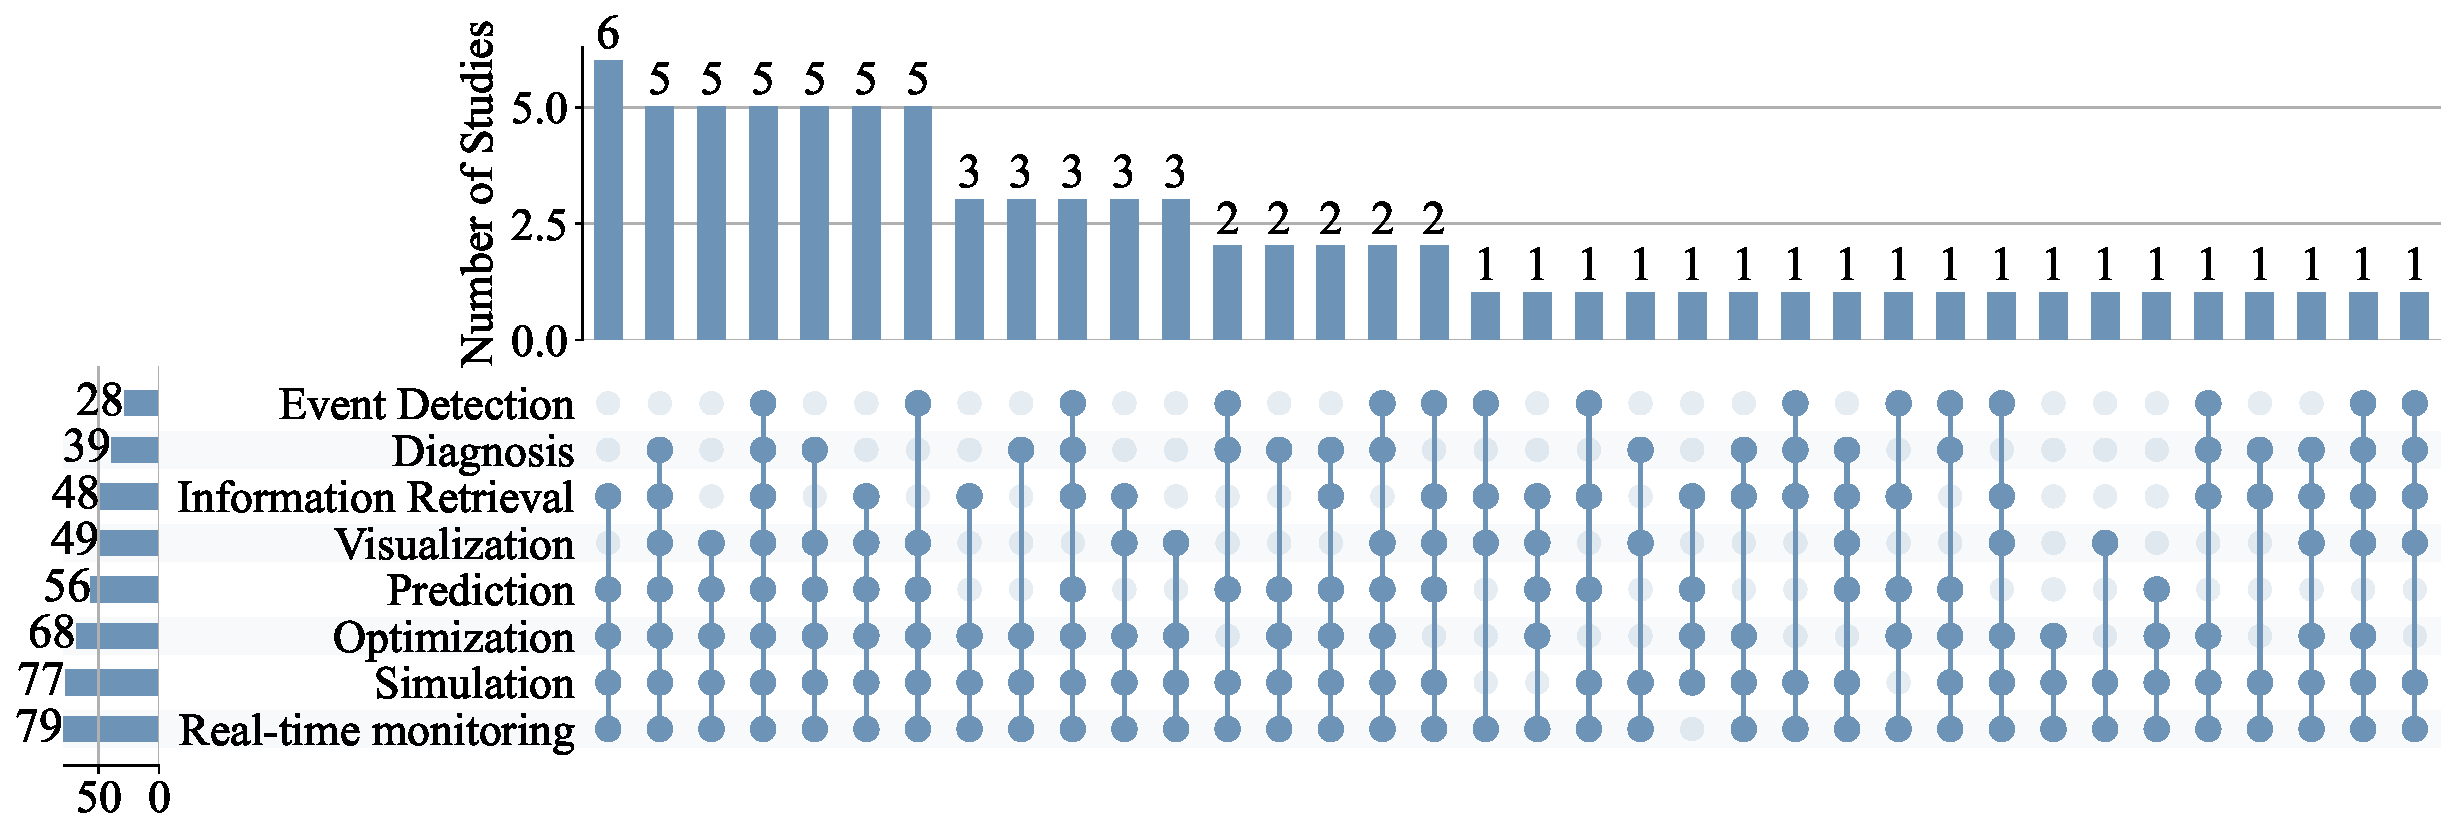
\includegraphics[width=\linewidth]{figures/Literature Review/rq3/dtServices.pdf}
    \caption{Combinations of DT services supported across reviewed SoTS studies}
    \label{fig:dt-services}
\end{figure*}
As shown in \figref{fig:dt-services}, DTs in SoTS commonly provide multiple services. Real-time monitoring, simulation, and optimization are the most frequently combined capabilities. Prediction, visualization, and information retrieval are also widely used, often appearing alongside these services. Common combinations include monitoring with simulation or prediction, with additional services such as diagnosis or event detection appearing in more specialized cases.

\subsubsection{Modeling and simulation formalisms and techniques}\label{sec:modeling-methods}

\begin{table*}[]
\centering
\setlength{\tabcolsep}{1em}
\caption{Modeling and simulation formalisms}
\label{tab:modeling-methods-structured-table}
\scriptsize
\begin{tabular}{@{}p{5cm} l p{7.5cm}@{}}
\toprule
\textbf{Category} & \textbf{Frequency} & \textbf{Studies} \\
\midrule
\textbf{Architectural and Structural} & \textbf{\maindatabar{31}} & \\
\;\;\corner{} Systems Modeling Language (SysML) & \subdatabar{13} & \cite{ashtaritalkhestani2019architecture,dahmen2022modeling,dickopf2019holistic,gollner2022collaborative,jiang2022novel,kutzke2021subsystem,lopez2023modeling,parri2019jarvis,parri2021framework,pickering2023towards,schluse2017experimentable,wagner2023using,zhang2022multi-scale} \\
\;\;\corner{} Unified Modeling Language (UML) & \subdatabar{12} & \cite{dahmen2022modeling,duan2023digital,gil2024integrating,gill2022method,gollner2022collaborative,heithoff2023challenges,hofmeister2024semantic,jiang2022novel,lee2022simulation,parri2019jarvis,parri2021framework,vogel-heuser2021approach} \\
\;\;\corner{} Business Process Modeling (BPM) & \subdatabar{3} & \cite{binder2021utilizing,kulkarni2019towards,vogel-heuser2021approach} \\
\;\;\corner{} Building Information Modeling (BIM) & \subdatabar{3} & \cite{coupaye2023graph-based,doubell2023digital,larsen2024towards} \\
\;\;\corner{} Subject-Oriented Modeling (S-BPM) & \subdatabar{2} & \cite{heininger2021capturing,stary2022privacy} \\
\;\;\corner{} State Models & \subdatabar{2} & \cite{kruger2022towards,reiche2021digital} \\
\;\;\corner{} \textit{Other} & \subdatabar{8} & \cite{binder2021utilizing,dahmen2022modeling,dobie2024network,gil2024integrating,gollner2022collaborative,kulkarni2019towards,villalonga2021decision-making,wagner2023using} \\
\textbf{Spatial and Visual Modeling} & \textbf{\maindatabar{24}} & \\
\;\;\corner{} Computer-Aided Design (CAD) & \subdatabar{12} & \cite{ashtaritalkhestani2019architecture,becue2018cyberfactory,coupaye2023graph-based,duan2023digital,ehemann2023digital,jiang2022novel,joseph2021aggregated,liu2020web-based,novak2022digitalized,park2020digital,reiche2021digital,zhang2021bi-level} \\
\;\;\corner{} 3D Modeling & \subdatabar{10} & \cite{bao2024digital,chavezbaliguat2023digital,ehemann2023digital,hatledal2020co-simulation,malayjerdi2022combined,mavromatis2024umbrella,priyanta2024is,samak2023autodrive,somma2023digital,vermesan2021internet} \\
\;\;\corner{} Geometric Models & \subdatabar{2} & \cite{duan2023digital,ehemann2023digital} \\
\;\;\corner{} Parametric Models & \subdatabar{2} & \cite{li2024comprehensive,wagner2023using} \\
\;\;\corner{} \textit{Other} & \subdatabar{6} & \cite{becue2018cyberfactory,chavezbaliguat2023digital,coupaye2023graph-based,demir2023vertically-integrated,ehemann2023digital,priyanta2024is} \\
\textbf{Mathematical and Statistical} & \textbf{\maindatabar{23}} & \\
\;\;\corner{} Bayesian Networks (BN) & \subdatabar{5} & \cite{alam2017c2ps,kutzke2021subsystem,lippi2023enabling,maheshwari2022digital,vogel-heuser2021approach} \\
\;\;\corner{} General Mathematical Models & \subdatabar{5} & \cite{hatledal2020co-simulation,howard2021greenhouse,jiang2022novel,kruger2022towards,maheshwari2022digital} \\
\;\;\corner{} Fuzzy Logic & \subdatabar{2} & \cite{alam2017c2ps,altamiranda2019system} \\
\;\;\corner{} Model Reference Adaptive Control (MRAC) & \subdatabar{2} & \cite{clark2021chapter,kulkarni2019towards} \\
\;\;\corner{} \textit{Other} & \subdatabar{18} & \cite{altamiranda2019system,barden2022academic,bertoni2022digital,chavezbaliguat2023digital,dobie2024network,esterle2021digital,folds2019digital,gil2023modeling,gill2022method,heininger2021capturing,howard2021greenhouse,jiang2022novel,kulkarni2019towards,lippi2023enabling,maheshwari2022digital,pillai2023digital,saraeian2022digital,vogel-heuser2021approach} \\
\textbf{Ontological and Knowledge Representation} & \textbf{\maindatabar{19}} & \\
\;\;\corner{} Web Ontology Language (OWL) & \subdatabar{7} & \cite{ashtaritalkhestani2019architecture,bao2024digital,gil2023modeling,hofmeister2024semantic,jiang2022novel,li2024comprehensive,liu2020web-based} \\
\;\;\corner{} AutomationML & \subdatabar{5} & \cite{ashtaritalkhestani2019architecture,gil2023modeling,gollner2022collaborative,liu2020web-based,novak2022digitalized} \\
\;\;\corner{} Resource Description Framework (RDF) & \subdatabar{3} & \cite{coupaye2023graph-based,hofmeister2024semantic,li2024comprehensive} \\
\;\;\corner{} Property Graphs (PGs) & \subdatabar{2} & \cite{coupaye2023graph-based,mahoro2023articulating} \\
\;\;\corner{} Information Model & \subdatabar{2} & \cite{hatledal2020co-simulation,reiche2021digital} \\
\;\;\corner{} \textit{Other} & \subdatabar{10} & \cite{coupaye2023graph-based,demir2023vertically-integrated,gil2023modeling,hofmeister2024cross-domain,hofmeister2024semantic,li2022cognitive,li2024comprehensive,monsalve2021novel,park2020digital,pickering2023towards} \\
\textbf{Formal and State Based Methods} & \textbf{\maindatabar{14}} & \\
\;\;\corner{} Finite State Machines (FSM) & \subdatabar{5} & \cite{alam2017c2ps,dahmen2022modeling,liu2020web-based,savur2019hrc-sos,vogel-heuser2021approach} \\
\;\;\corner{} Fault Tree Analysis (FTA) & \subdatabar{3} & \cite{parri2019jarvis,parri2021framework,saraeian2022digital} \\
\;\;\corner{} \textit{Other} & \subdatabar{7} & \cite{chen2018digital,hatledal2020co-simulation,heininger2021capturing,heithoff2023challenges,larsen2024towards,oquendo2019dealing,parri2019jarvis} \\
\textbf{AI and Machine Learning} & \textbf{\maindatabar{13}} & \\
\;\;\corner{} Machine Learning & \subdatabar{4} & \cite{dobie2024network,esterle2021digital,folds2019digital,jiang2022novel} \\
\;\;\corner{} Reinforcement Learning (RL) & \subdatabar{2} & \cite{clark2021chapter,kulkarni2019towards} \\
\;\;\corner{} Genetic Algorithms (GA) & \subdatabar{2} & \cite{kutzke2021subsystem,park2020digital} \\
\;\;\corner{} \textit{Other} & \subdatabar{5} & \cite{altamiranda2019system,bao2024digital,chen2018digital,saraeian2022digital,villalonga2021decision-making} \\
\textbf{Continuous Simulation} & \textbf{\maindatabar{12}} & \\
\;\;\corner{} System Dynamics Models (SDM) & \subdatabar{4} & \cite{folds2019digital,gill2022method,kulkarni2019towards,pickering2023towards} \\
\;\;\corner{} Kinematic Models & \subdatabar{3} & \cite{duan2023digital,gil2023modeling,schluse2017experimentable} \\
\;\;\corner{} General Physics Models & \subdatabar{2} & \cite{demir2023vertically-integrated,hatakeyama2018systems} \\
\;\;\corner{} Finite Element Method (FEM) & \subdatabar{2} & \cite{demir2023vertically-integrated,li2024comprehensive} \\
\;\;\corner{} \textit{Other} & \subdatabar{4} & \cite{altamiranda2019system,demir2023vertically-integrated,gil2023modeling,monsalve2021novel} \\
\textbf{Agent-Based Simulation} & \textbf{\maindatabar{10}} & \\
\;\;\corner{} Multi Agent System (MAS) & \subdatabar{9} & \cite{clark2021chapter,heininger2021capturing,howard2021greenhouse,jirsa2024use,liu2020web-based,marah2023architecture,samak2023autodrive,vogel-heuser2021approach,zhang2021bi-level} \\
\;\;\corner{} Agent Based Modeling (ABM) & \subdatabar{2} & \cite{barden2022academic,clark2021chapter} \\
\;\;\corner{} \textit{Other} & \subdatabar{1} & \cite{marah2023architecture} \\
\textbf{Discrete-Event Simulation} & \textbf{\maindatabar{8}} & \\
\;\;\corner{} Discrete Event Simulation (DES) & \subdatabar{4} & \cite{bertoni2022digital,clark2021chapter,demir2023vertically-integrated,villalonga2021decision-making} \\
\;\;\corner{} Discrete Event System Specification (DEVS) & \subdatabar{2} & \cite{lee2022simulation,oquendo2019dealing} \\
\;\;\corner{} \textit{Other} & \subdatabar{3} & \cite{lee2022simulation,wang2024construction,zhang2022multi-scale} \\
\bottomrule
\end{tabular}
\end{table*}
As shown in \tabref{tab:modeling-methods-structured-table}, architectural and structural modeling approaches are the most commonly used, with UML and SysML supporting system specification. Visual and spatial models, such as CAD and 3D representations, are also used to represent physical structure. Mathematical and statistical models are used to capture system dynamics and uncertainty, while ontological methods support semantic integration. Formal methods and AI/ML approaches appear less frequently and are used for verification and adaptive behavior.

\begin{conclusionframe}{RQ3: Characteristics of DTs in SoTS}
Most SoTS use fully autonomous DTs that provide monitoring, simulation, prediction, and optimization services. Modeling approaches used most frequently are architectural, visual, and mathematical formalisms.
\end{conclusionframe}

\subsection{What are the characteristics of SoS that are combined with DTs? (RQ4)}\label{results-rq4}

To identify the characteristics of SoS used in SoTS, we analyze their supported SoS dimensions and the forms of emergent behavior they exhibit.

\subsubsection{Dimensions of SoS}\label{sec:dimensions}

\begin{figure*}[htb]
    \centering
     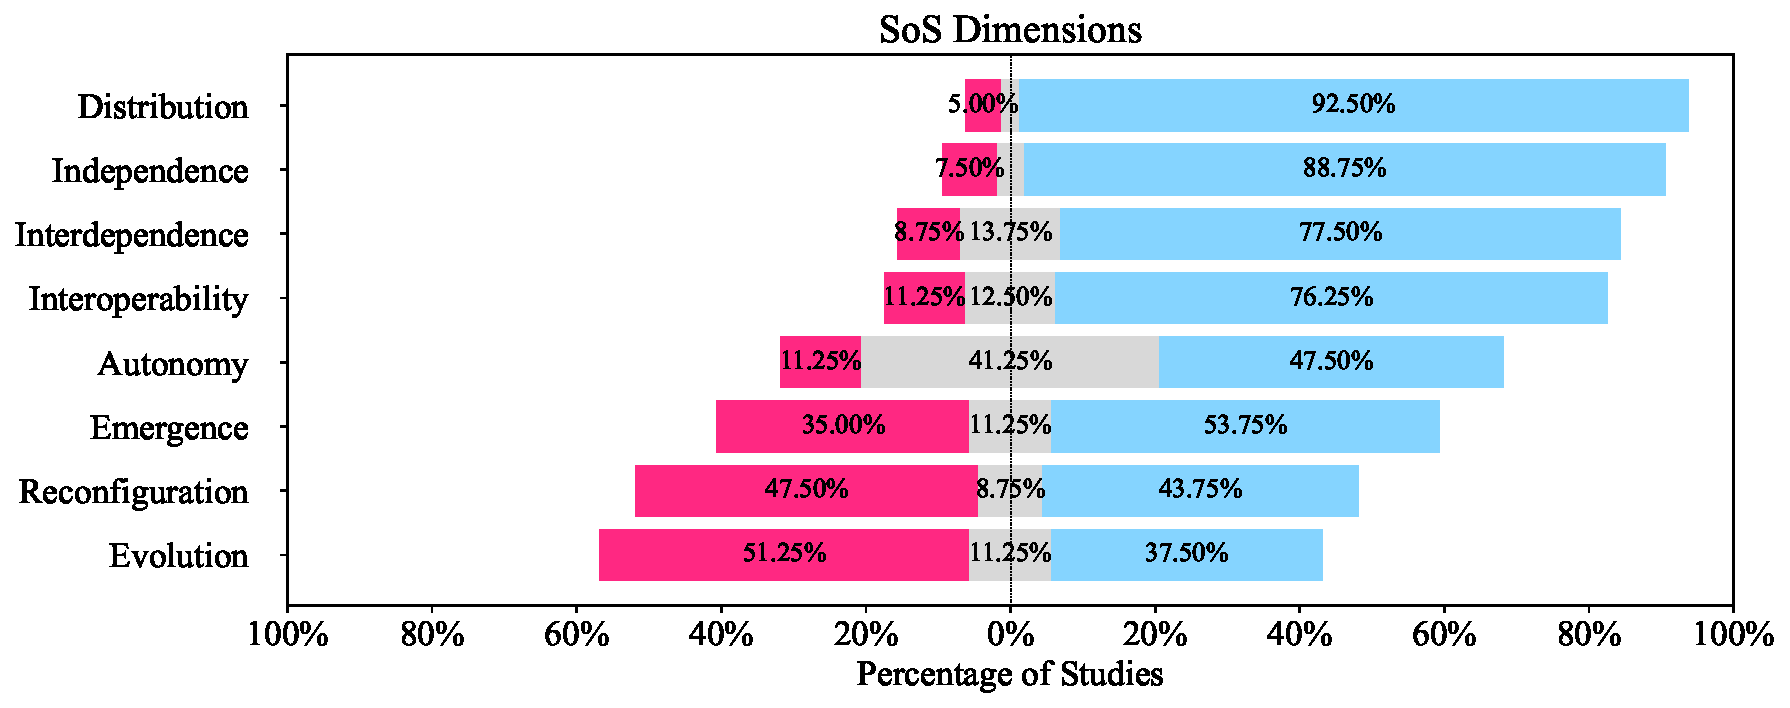
\includegraphics[width=\linewidth]{figures/Literature Review/rq4/sosDimensions.pdf}
    \caption[SoS dimensions]{SoS dimensions: 
     {\color[HTML]{ff2882}\ding{108}} No,  
     {\color[HTML]{d8d8d8}\ding{108}} Partial, 
     {\color[HTML]{85d4ff}\ding{108}} Yes
    } 
    \label{fig:sos-dim}
\end{figure*}

\figref{fig:sos-dim} shows the SoS dimensions addressed in the studies. Distribution and independence are the most consistently represented dimensions, indicating that SoTS commonly involve geographically dispersed and operationally independent constituents. Interdependence and interoperability also appear frequently, reflecting the importance of coordination and information exchange between constituent systems. Autonomy and emergence are less consistently addressed, often appearing only partially in the analyzed studies. Reconfiguration and evolution are the least represented dimensions, suggesting that dynamic system adaptation and long-term system evolution are not widely incorporated in current SoTS implementations.

\subsubsection{Emergence type}\label{sec:emergence-type}
\begin{table*}[]
            \centering
            \footnotesize
            \caption{Emergence type}
            \label{tab:emergence-type-table}
            \begin{tabular}{@{}p{4cm}l p{8.5cm}@{}}
            \toprule
            \multicolumn{1}{c}{\textbf{Emergence}} & 
            \multicolumn{1}{c}{\textbf{Frequency}} & 
            \multicolumn{1}{c}{\textbf{Studies}} \\ 
            \midrule
            Not Addressed & \maindatabar{28} & \cite{acharya2023twins,ashtaritalkhestani2019architecture,aziz2022empowering,becue2018cyberfactory,binder2021utilizing,chavezbaliguat2023digital,doubell2023digital,duan2023digital,gil2023modeling,gollner2022collaborative,hatakeyama2018systems,hatledal2020co-simulation,heithoff2023challenges,hofmeister2024semantic,howard2021greenhouse,human2023design,kruger2022towards,kutzke2021subsystem,li2024comprehensive,liu2020web-based,mahoro2023articulating,marah2023architecture,monsalve2021novel,redelinghuys2020six-layer,reiche2021digital,villalonga2021decision-making,vogel-heuser2021approach,zhang2021bi-level} \\
Simple & \maindatabar{16} & \cite{gil2024integrating,lee2022simulation,li2022cognitive,lopez2023modeling,maheshwari2022digital,novak2022digitalized,park2020digital,parri2021framework,pillai2023digital,potteiger2023live,priyanta2024is,samak2023autodrive,somma2023digital,vermesan2021internet,wagner2023using,zhang2022multi-scale} \\
Weak & \maindatabar{30} & \cite{alam2017c2ps,altamiranda2019system,bao2024digital,barden2022academic,bellavista2023requirements,bertoni2022digital,chen2018digital,clark2021chapter,coupaye2023graph-based,demir2023vertically-integrated,dickopf2019holistic,dobie2024network,ehemann2023digital,esterle2021digital,gill2022method,heininger2021capturing,hofmeister2024cross-domain,larsen2024towards,lippi2023enabling,malayjerdi2022combined,mavromatis2024umbrella,oquendo2019dealing,parri2019jarvis,pickering2023towards,saraeian2022digital,savur2019hrc-sos,schluse2017experimentable,stary2022privacy,wang2024construction,wullink2024foundational} \\
Strong & \maindatabar{6} & \cite{dahmen2022modeling,folds2019digital,jiang2022novel,jirsa2024use,joseph2021aggregated,kulkarni2019towards} \\
\bottomrule
            \end{tabular}
            \end{table*}
As shown in \tabref{tab:emergence-type-table}, weak emergence is the most commonly reported form of emergent behavior and is typically observed through system-level simulations where behaviors arise from interactions among components \cite{malayjerdi2022combined}. Simple emergence appears in systems with predictable interactions, such as coordinated shop floor operations \cite{zhang2022multi-scale}. Strong emergence is addressed less frequently and is observed in domains such as mining and automotive systems \cite{bertoni2022digital, dahmen2022modeling}. 

\begin{conclusionframe}{RQ4: Characteristics of SoS in SoTS}
SoTS support architectural SoS dimensions (distribution, independence, interdependence, and interoperability) but less frequently include emergence, reconfiguration, and evolution. Emergent behavior is addressed in two thirds of the studies, most often as weak emergence, and many studies do not consider emergence at all.
\end{conclusionframe}




\subsection{How are non-functional properties addressed in systems that combine SoS and DT? (RQ5)}\label{results-rq5}

To understand how non-functional properties---specifically reliability and security---are handled in SoTS, we analyze whether these concerns are addressed at the system requirements, architecture, or implementation levels, and whether they are evaluated.

\begin{table*}[htp]
            \centering
            \footnotesize
            \caption{Reliability}
            \label{tab:reliability-table}
            \begin{tabular}{@{}p{4cm}l p{8.5cm}@{}}
            \toprule
            \multicolumn{1}{c}{\textbf{Context}} & 
            \multicolumn{1}{c}{\textbf{Frequency}} & 
            \multicolumn{1}{c}{\textbf{Studies}} \\ 
            \midrule
            Not Addressed & \maindatabar{26} & \cite{bao2024digital,bertoni2022digital,binder2021utilizing,clark2021chapter,coupaye2023graph-based,dahmen2022modeling,demir2023vertically-integrated,dickopf2019holistic,ehemann2023digital,gil2023modeling,gil2024integrating,gollner2022collaborative,hatakeyama2018systems,jiang2022novel,li2022cognitive,li2024comprehensive,maheshwari2022digital,mahoro2023articulating,reiche2021digital,samak2023autodrive,schluse2017experimentable,somma2023digital,stary2022privacy,wagner2023using,wang2024construction,zhang2022multi-scale} \\
Mentioned & \maindatabar{8} & \cite{barden2022academic,becue2018cyberfactory,heininger2021capturing,jirsa2024use,lee2022simulation,marah2023architecture,pickering2023towards,wullink2024foundational} \\
Architecturally Addressed & \maindatabar{41} & \cite{acharya2023twins,alam2017c2ps,altamiranda2019system,ashtaritalkhestani2019architecture,aziz2022empowering,bellavista2023requirements,chavezbaliguat2023digital,chen2018digital,dobie2024network,doubell2023digital,duan2023digital,esterle2021digital,folds2019digital,gill2022method,hatledal2020co-simulation,heithoff2023challenges,hofmeister2024cross-domain,hofmeister2024semantic,howard2021greenhouse,human2023design,joseph2021aggregated,kruger2022towards,kulkarni2019towards,larsen2024towards,lippi2023enabling,liu2020web-based,lopez2023modeling,mavromatis2024umbrella,monsalve2021novel,novak2022digitalized,parri2021framework,parri2019jarvis,pillai2023digital,potteiger2023live,priyanta2024is,redelinghuys2020six-layer,savur2019hrc-sos,vermesan2021internet,villalonga2021decision-making,vogel-heuser2021approach,zhang2021bi-level} \\
Explicitly Modeled & \maindatabar{2} & \cite{kutzke2021subsystem,oquendo2019dealing} \\
Evaluated or Validated & \maindatabar{3} & \cite{malayjerdi2022combined,park2020digital,saraeian2022digital} \\
\bottomrule
            \end{tabular}
            \end{table*}
\begin{table*}[]
            \centering
            \footnotesize
            \caption{Security}
            \label{tab:security-table}
            \begin{tabular}{@{}p{4cm}l p{8.5cm}@{}}
            \toprule
            \multicolumn{1}{c}{\textbf{Context}} & 
            \multicolumn{1}{c}{\textbf{Frequency}} & 
            \multicolumn{1}{c}{\textbf{Studies}} \\ 
            \midrule
            Not Addressed & \maindatabar{32} & \cite{bertoni2022digital,chavezbaliguat2023digital,chen2018digital,clark2021chapter,dahmen2022modeling,dickopf2019holistic,ehemann2023digital,folds2019digital,gil2023modeling,gil2024integrating,gollner2022collaborative,hofmeister2024cross-domain,hofmeister2024semantic,howard2021greenhouse,kulkarni2019towards,kutzke2021subsystem,lee2022simulation,li2022cognitive,lippi2023enabling,lopez2023modeling,maheshwari2022digital,novak2022digitalized,oquendo2019dealing,park2020digital,pillai2023digital,priyanta2024is,samak2023autodrive,savur2019hrc-sos,schluse2017experimentable,wagner2023using,wang2024construction,zhang2022multi-scale} \\
Mentioned & \maindatabar{24} & \cite{alam2017c2ps,altamiranda2019system,ashtaritalkhestani2019architecture,bao2024digital,barden2022academic,bellavista2023requirements,binder2021utilizing,demir2023vertically-integrated,doubell2023digital,duan2023digital,esterle2021digital,gill2022method,hatakeyama2018systems,jirsa2024use,joseph2021aggregated,li2024comprehensive,mahoro2023articulating,marah2023architecture,monsalve2021novel,reiche2021digital,saraeian2022digital,vogel-heuser2021approach,wullink2024foundational,zhang2021bi-level} \\
Architecturally Addressed & \maindatabar{19} & \cite{acharya2023twins,coupaye2023graph-based,dobie2024network,hatledal2020co-simulation,heininger2021capturing,heithoff2023challenges,human2023design,jiang2022novel,kruger2022towards,larsen2024towards,liu2020web-based,parri2021framework,parri2019jarvis,pickering2023towards,potteiger2023live,redelinghuys2020six-layer,somma2023digital,vermesan2021internet,villalonga2021decision-making} \\
Explicitly Modeled & \maindatabar{2} & \cite{becue2018cyberfactory,stary2022privacy} \\
Evaluated or Validated & \maindatabar{3} & \cite{aziz2022empowering,malayjerdi2022combined,mavromatis2024umbrella} \\
\bottomrule
            \end{tabular}
            \end{table*}
As shown in \tabref{tab:reliability-table}, reliability is addressed in many studies, primarily at the architectural level. Common mechanisms include fallback to local or lightweight DTs during communication loss \cite{alam2017c2ps, larsen2024towards}, asynchronous communication to handle intermittent updates \cite{acharya2023twins, liu2020web-based}, and runtime fault recovery \cite{esterle2021digital, villalonga2021decision-making}. Only a small number of studies include formal modeling or validation of reliability, typically through simulation or fault injection \cite{park2020digital, saraeian2022digital}.

As shown in \tabref{tab:security-table}, security is addressed less frequently. It is typically implemented through architectural mechanisms such as secure communication, authentication, and access control \cite{aziz2022empowering, dobie2024network}. Explicit modeling and validation of security appear in only a few studies, using approaches such as threat simulation or attack injection \cite{malayjerdi2022combined, stary2022privacy}.

\begin{conclusionframe}{RQ5: NFPs focused on in SoTS}
Reliability is frequently addressed at the architectural level, but is rarely formalized or evaluated. Security is less commonly treated, and most studies lack explicit modeling or validation.
\end{conclusionframe}


\subsection{What is the level of technical and research maturity in SoTS? (RQ6)}\label{results-rq6}
To assess the maturity of SoTS research, we analyze technology readiness levels (TRLs), contribution types, evaluation strategies, and the use of standards.

\subsubsection{Technology readiness levels and contribution types}\label{sec:trl-contribution}

\begin{table*}[htp]
            \centering
            \scriptsize
            \caption{TRL}
            \label{tab:trl-table}
            \begin{tabular}{@{}p{4cm}l p{8.5cm}@{}}
            \toprule
            \multicolumn{1}{c}{\textbf{TRL}} & 
            \multicolumn{1}{c}{\textbf{Frequency}} & 
            \multicolumn{1}{c}{\textbf{Studies}} \\ 
            \midrule
            Initial & \maindatabar{20} & \cite{becue2018cyberfactory,folds2019digital,kruger2022towards,li2022cognitive,lippi2023enabling,lopez2023modeling,maheshwari2022digital,mahoro2023articulating,oquendo2019dealing,parri2021framework,parri2019jarvis,pillai2023digital,samak2023autodrive,saraeian2022digital,somma2023digital,stary2022privacy,vermesan2021internet,wagner2023using,wang2024construction,wullink2024foundational} \\
Proof-of-Concept & \maindatabar{16} & \cite{acharya2023twins,alam2017c2ps,altamiranda2019system,barden2022academic,demir2023vertically-integrated,dobie2024network,esterle2021digital,gollner2022collaborative,hatakeyama2018systems,hatledal2020co-simulation,heininger2021capturing,hofmeister2024cross-domain,joseph2021aggregated,redelinghuys2020six-layer,reiche2021digital,villalonga2021decision-making} \\
Demo Prototype & \maindatabar{35} & \cite{aziz2022empowering,bao2024digital,bellavista2023requirements,bertoni2022digital,chavezbaliguat2023digital,chen2018digital,clark2021chapter,dahmen2022modeling,dickopf2019holistic,doubell2023digital,duan2023digital,gil2023modeling,gil2024integrating,gill2022method,heithoff2023challenges,howard2021greenhouse,human2023design,jiang2022novel,jirsa2024use,kulkarni2019towards,kutzke2021subsystem,larsen2024towards,lee2022simulation,li2024comprehensive,liu2020web-based,marah2023architecture,monsalve2021novel,pickering2023towards,potteiger2023live,priyanta2024is,savur2019hrc-sos,schluse2017experimentable,vogel-heuser2021approach,zhang2022multi-scale,zhang2021bi-level} \\
Deployed Prototype & \maindatabar{8} & \cite{ashtaritalkhestani2019architecture,binder2021utilizing,coupaye2023graph-based,ehemann2023digital,hofmeister2024semantic,malayjerdi2022combined,novak2022digitalized,park2020digital} \\
Operational & \maindatabar{1} & \cite{mavromatis2024umbrella} \\
\bottomrule
            \end{tabular}
            \end{table*}
\begin{table*}[]
            \centering
            \footnotesize
            \caption{Contribution type}
            \label{tab:contribution-type-table}
            \begin{tabular}{@{}p{4cm}l p{8.5cm}@{}}
            \toprule
            \multicolumn{1}{c}{\textbf{Contribution}} & 
            \multicolumn{1}{c}{\textbf{Frequency}} & 
            \multicolumn{1}{c}{\textbf{Studies}} \\ 
            \midrule
            Technical & \maindatabar{60} & \cite{acharya2023twins,alam2017c2ps,aziz2022empowering,bao2024digital,barden2022academic,bellavista2023requirements,bertoni2022digital,chavezbaliguat2023digital,chen2018digital,clark2021chapter,dahmen2022modeling,demir2023vertically-integrated,dickopf2019holistic,doubell2023digital,duan2023digital,ehemann2023digital,gil2023modeling,gil2024integrating,gollner2022collaborative,hatledal2020co-simulation,heininger2021capturing,heithoff2023challenges,hofmeister2024cross-domain,hofmeister2024semantic,howard2021greenhouse,jiang2022novel,jirsa2024use,kulkarni2019towards,kutzke2021subsystem,larsen2024towards,lee2022simulation,li2022cognitive,li2024comprehensive,lippi2023enabling,liu2020web-based,lopez2023modeling,maheshwari2022digital,mahoro2023articulating,marah2023architecture,monsalve2021novel,novak2022digitalized,oquendo2019dealing,park2020digital,parri2021framework,parri2019jarvis,pickering2023towards,pillai2023digital,potteiger2023live,priyanta2024is,reiche2021digital,samak2023autodrive,saraeian2022digital,savur2019hrc-sos,schluse2017experimentable,somma2023digital,stary2022privacy,villalonga2021decision-making,vogel-heuser2021approach,wagner2023using,zhang2021bi-level} \\
Conceptual & \maindatabar{13} & \cite{altamiranda2019system,becue2018cyberfactory,dobie2024network,esterle2021digital,folds2019digital,hatakeyama2018systems,human2023design,joseph2021aggregated,kruger2022towards,redelinghuys2020six-layer,vermesan2021internet,wang2024construction,wullink2024foundational} \\
Case Study & \maindatabar{7} & \cite{ashtaritalkhestani2019architecture,binder2021utilizing,coupaye2023graph-based,gill2022method,malayjerdi2022combined,mavromatis2024umbrella,zhang2022multi-scale} \\
\bottomrule
            \end{tabular}
            \end{table*}
As shown in \tabref{tab:trl-table}, most studies are positioned at low-to-mid maturity levels, with demonstrative prototypes and proof-of-concept implementations being the most common. Deployed or fully operational systems appear only rarely. In \tabref{tab:contribution-type-table}, technical contributions are the most common, typically proposing architectures, frameworks, or implementations. Conceptual works appear less frequently, and case studies are limited. \figref{fig:trl-v-cont} shows that technical contributions appear across all maturity levels, while conceptual works are concentrated at lower TRLs. Case studies appear primarily at higher maturity levels.

\begin{figure*}[htb]
    \centering
    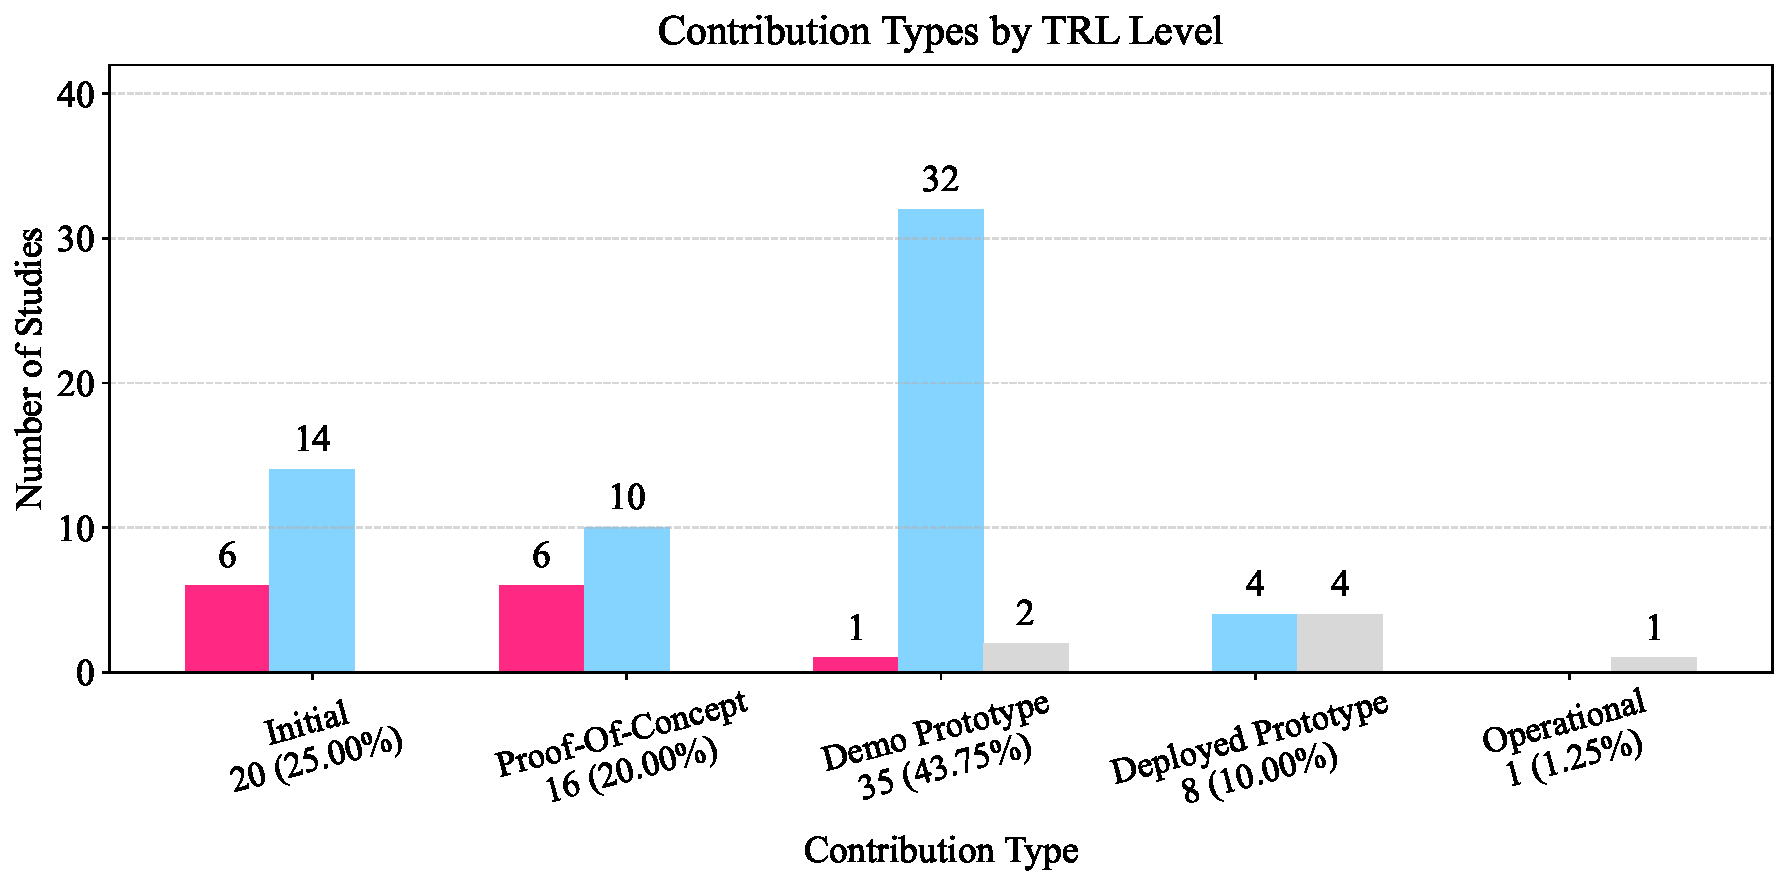
\includegraphics[width=0.9\linewidth]{figures/Literature Review/rq6/trlVsContributionType.pdf}
    \caption{Distribution of contribution types across TRLs}
    \caption*{{
    \color[HTML]{FF2882}\ding{110}} Conceptual
    ~~~{\color[HTML]{85d4ff}\ding{110}} Technical
    ~~~{\color[HTML]{d8d8d8}\ding{110}} Case Study
    }
    \label{fig:trl-v-cont}
\end{figure*}


\subsubsection{Evaluation}\label{sec:literature-review-evaluation}
\begin{table*}[htp]
\centering
\setlength{\tabcolsep}{1em}
\caption{Validation and evaluation approaches}
\label{tab:evaluation-structured-table}
\scriptsize
\begin{tabular}{@{}p{5cm} l p{7cm}@{}}
\toprule
\textbf{Evaluation Category} & \textbf{Frequency} & \textbf{Studies} \\
\midrule
\textbf{Validation} & \textbf{\maindatabar{72}} & \\
\;\;\corner{} Prototyping & \subdatabar{36} & \cite{aziz2022empowering,bao2024digital,bellavista2023requirements,chavezbaliguat2023digital,dahmen2022modeling,doubell2023digital,duan2023digital,ehemann2023digital,gil2023modeling,gollner2022collaborative,heininger2021capturing,heithoff2023challenges,hofmeister2024semantic,howard2021greenhouse,jiang2022novel,jirsa2024use,larsen2024towards,li2022cognitive,li2024comprehensive,liu2020web-based,lopez2023modeling,marah2023architecture,monsalve2021novel,novak2022digitalized,oquendo2019dealing,park2020digital,parri2019jarvis,parri2021framework,pickering2023towards,reiche2021digital,samak2023autodrive,saraeian2022digital,somma2023digital,stary2022privacy,villalonga2021decision-making,wagner2023using} \\
\;\;\corner{} Empirical Simulation & \subdatabar{16} & \cite{barden2022academic,chen2018digital,clark2021chapter,demir2023vertically-integrated,dickopf2019holistic,hatledal2020co-simulation,hofmeister2024cross-domain,kulkarni2019towards,lee2022simulation,lippi2023enabling,maheshwari2022digital,pillai2023digital,potteiger2023live,schluse2017experimentable,vogel-heuser2021approach,zhang2021bi-level} \\
\;\;\corner{} Architectural/Conceptual Design & \subdatabar{13} & \cite{altamiranda2019system,becue2018cyberfactory,dobie2024network,esterle2021digital,folds2019digital,hatakeyama2018systems,human2023design,joseph2021aggregated,kruger2022towards,redelinghuys2020six-layer,vermesan2021internet,wang2024construction,wullink2024foundational} \\
\;\;\corner{} Laboratory Experiments & \subdatabar{4} & \cite{acharya2023twins,gil2024integrating,priyanta2024is,savur2019hrc-sos} \\
\;\;\corner{} Mathematical Analysis & \subdatabar{3} & \cite{alam2017c2ps,kutzke2021subsystem,mahoro2023articulating} \\
\textbf{Evaluation} & \textbf{\maindatabar{8}} & \\
\;\;\corner{} Industrial Case Study & \subdatabar{7} & \cite{ashtaritalkhestani2019architecture,binder2021utilizing,coupaye2023graph-based,gill2022method,malayjerdi2022combined,mavromatis2024umbrella,zhang2022multi-scale} \\
\;\;\corner{} Action Research & \subdatabar{1} & \cite{bertoni2022digital} \\
\bottomrule
\end{tabular}
\end{table*}
As shown in \tabref{tab:evaluation-structured-table}, prototyping and simulation are the most commonly used evaluation approaches. Simulation is used to assess system behavior under controlled conditions, while prototyping demonstrates feasibility in implemented systems \cite{hatledal2020co-simulation, larsen2024towards}. Other methods appear less frequently, including laboratory experiments and mathematical analysis. These are used to assess physical system behavior, such as human-robot interaction, and to formalize system properties \cite{savur2019hrc-sos, mahoro2023articulating}. Studies involving real-world deployment or empirical validation also appear less frequently. These include industrial case studies and action research in operational environments \cite{ashtaritalkhestani2019architecture, bertoni2022digital}.


\subsubsection{Standards}\label{sec:standards}
\begin{table*}[]
            \centering
            \footnotesize
            \caption{Standards}
            \label{tab:standards-table}
            \begin{tabular}{@{}p{4cm}l p{8.5cm}@{}}
            \toprule
            \multicolumn{1}{c}{\textbf{Standard}} & 
            \multicolumn{1}{c}{\textbf{Frequency}} & 
            \multicolumn{1}{c}{\textbf{Studies}} \\ 
            \midrule
            Open Platform Communications Unified Architecture (OPC UA) & \maindatabar{13} & \cite{acharya2023twins,ashtaritalkhestani2019architecture,binder2021utilizing,dobie2024network,gollner2022collaborative,howard2021greenhouse,jirsa2024use,joseph2021aggregated,liu2020web-based,novak2022digitalized,redelinghuys2020six-layer,reiche2021digital,villalonga2021decision-making} \\
IEC 63278: Asset Administration Shell & \maindatabar{8} & \cite{acharya2023twins,ashtaritalkhestani2019architecture,gil2023modeling,gill2022method,gollner2022collaborative,jirsa2024use,reiche2021digital,vogel-heuser2021approach} \\
Reference Architectural Model Industrie 4.0 (RAMI 4.0) & \maindatabar{4} & \cite{binder2021utilizing,gill2022method,human2023design,park2020digital} \\
Other & \maindatabar{26} & \cite{alam2017c2ps,altamiranda2019system,ashtaritalkhestani2019architecture,barden2022academic,bellavista2023requirements,binder2021utilizing,dickopf2019holistic,dobie2024network,gollner2022collaborative,hatledal2020co-simulation,heininger2021capturing,heithoff2023challenges,howard2021greenhouse,human2023design,jiang2022novel,li2022cognitive,malayjerdi2022combined,monsalve2021novel,novak2022digitalized,parri2019jarvis,parri2021framework,pickering2023towards,savur2019hrc-sos,stary2022privacy,vermesan2021internet,vogel-heuser2021approach} \\
\bottomrule
            \end{tabular}
            \end{table*}
\begin{table*}[htp]
            \centering
            \scriptsize
            \caption{Standards usage context (DT vs. SoS)}
            \label{tab:dt-or-sos-related-table}
            \begin{tabular}{@{}p{4cm}l p{8.5cm}@{}}
            \toprule
            \multicolumn{1}{c}{\textbf{Context}} & 
            \multicolumn{1}{c}{\textbf{Frequency}} & 
            \multicolumn{1}{c}{\textbf{Studies}} \\ 
            \midrule
            DT & \maindatabar{18} & \cite{acharya2023twins,alam2017c2ps,bellavista2023requirements,binder2021utilizing,dickopf2019holistic,gil2023modeling,gill2022method,gollner2022collaborative,hatledal2020co-simulation,heininger2021capturing,heithoff2023challenges,jirsa2024use,joseph2021aggregated,liu2020web-based,malayjerdi2022combined,reiche2021digital,stary2022privacy,villalonga2021decision-making} \\
SoS & \maindatabar{10} & \cite{altamiranda2019system,barden2022academic,howard2021greenhouse,li2022cognitive,monsalve2021novel,park2020digital,pickering2023towards,redelinghuys2020six-layer,savur2019hrc-sos,vermesan2021internet} \\
Both & \maindatabar{6} & \cite{ashtaritalkhestani2019architecture,dobie2024network,human2023design,jiang2022novel,novak2022digitalized,vogel-heuser2021approach} \\
\bottomrule
            \end{tabular}
            \end{table*}
As shown in \tabref{tab:standards-table}, standards are referenced inconsistently across studies. OPC UA is the most commonly used standard. IEC 63278 and RAMI 4.0 also appear in several studies. Other standards, including domain-specific and security-related ones such as GDPR and OAuth 2.0, appear less frequently. As shown in \tabref{tab:dt-or-sos-related-table}, most standards are applied in DT-specific contexts, with fewer addressing SoS concerns or both layers simultaneously.

\begin{conclusionframe}{RQ6: Maturity of SoTS research}
Most studies are positioned at low-to-mid TRLs, with demo prototypes and proof-of-concept efforts being the most common. Validation is primarily conducted through prototyping and simulation, with limited empirical evaluation. Standards are inconsistently applied and tend to focus on DT-specific components, with few addressing SoS integration or supporting both layers.
\end{conclusionframe}


\subsection{What technology is used to implement systems that combine SoS and DT? (RQ7)}\label{results-rq7}

To understand what technologies support the implementation of SoTS, we examine the programming languages and data formats used, as well as the development frameworks and platforms adopted across studies.

\subsubsection{Programming languages and formats}\label{sec:programming-languages}
\begin{table*}[]
\centering
\setlength{\tabcolsep}{1em}
\caption{Programming languages and data formats}
\label{tab:programming-languages-structured-table}
\scriptsize
\begin{tabular}{@{}p{5cm} l p{7.5cm}@{}}
\toprule
\textbf{Category} & \textbf{Frequency} & \textbf{Studies} \\
\midrule
\textbf{General Purpose} & \textbf{\maindatabar{36}} & \\
\;\;\corner{} Python & \subdatabar{22} & \cite{bao2024digital,barden2022academic,bellavista2023requirements,chavezbaliguat2023digital,doubell2023digital,duan2023digital,gil2023modeling,jirsa2024use,lippi2023enabling,liu2020web-based,maheshwari2022digital,malayjerdi2022combined,marah2023architecture,mavromatis2024umbrella,monsalve2021novel,park2020digital,potteiger2023live,samak2023autodrive,saraeian2022digital,savur2019hrc-sos,vogel-heuser2021approach,wagner2023using} \\
\;\;\corner{} Java & \subdatabar{14} & \cite{alam2017c2ps,ashtaritalkhestani2019architecture,aziz2022empowering,bellavista2023requirements,clark2021chapter,gil2023modeling,gil2024integrating,hatledal2020co-simulation,li2024comprehensive,marah2023architecture,parri2019jarvis,parri2021framework,vogel-heuser2021approach,wagner2023using} \\
\;\;\corner{} JavaScript & \subdatabar{8} & \cite{bao2024digital,barden2022academic,doubell2023digital,duan2023digital,hofmeister2024semantic,liu2020web-based,priyanta2024is,samak2023autodrive} \\
\;\;\corner{} C++ & \subdatabar{4} & \cite{hatledal2020co-simulation,mavromatis2024umbrella,park2020digital,samak2023autodrive} \\
\;\;\corner{} C\# & \subdatabar{3} & \cite{lee2022simulation,park2020digital,redelinghuys2020six-layer} \\
\;\;\corner{} C & \subdatabar{1} & \cite{hatledal2020co-simulation} \\
\;\;\corner{} Xtend & \subdatabar{1} & \cite{oquendo2019dealing} \\
\;\;\corner{} Jython & \subdatabar{1} & \cite{wagner2023using} \\
\textbf{Data Representation} & \textbf{\maindatabar{12}} & \\
\;\;\corner{} XML & \subdatabar{9} & \cite{ashtaritalkhestani2019architecture,binder2021utilizing,dahmen2022modeling,jiang2022novel,jirsa2024use,kutzke2021subsystem,monsalve2021novel,oquendo2019dealing,redelinghuys2020six-layer} \\
\;\;\corner{} JSON & \subdatabar{5} & \cite{acharya2023twins,aziz2022empowering,dahmen2022modeling,jirsa2024use,vogel-heuser2021approach} \\
\textbf{Markup and Styling} & \textbf{\maindatabar{4}} & \\
\;\;\corner{} HTML & \subdatabar{4} & \cite{bao2024digital,doubell2023digital,hofmeister2024semantic,samak2023autodrive} \\
\;\;\corner{} CSS & \subdatabar{4} & \cite{bao2024digital,doubell2023digital,hofmeister2024semantic,samak2023autodrive} \\
\bottomrule
\end{tabular}
\end{table*} 
As shown in \tabref{tab:programming-languages-structured-table}, most studies use general-purpose programming languages, particularly Python and Java. Languages such as JavaScript, C++, and C\# appear less frequently. Structured data formats, including XML and JSON, are commonly used for data exchange between system components. Markup and styling languages, such as HTML and CSS, are used primarily for visualization and interface development.

\subsubsection{Frameworks and platforms}\label{sec:frameworks}
\begin{table*}[]
\centering
\setlength{\tabcolsep}{1em}
\caption{Tools and frameworks}
\label{tab:frameworks-structured-table}
\scriptsize
\begin{tabular}{@{}p{5cm} l p{7.5cm}@{}}
\toprule
\textbf{Category} & \textbf{Frequency} & \textbf{Studies} \\
\midrule
\textbf{Modeling \& Simulation} & \textbf{\maindatabar{35}} & \\
\;\;\corner{} MATLAB & \subdatabar{10} & \cite{ashtaritalkhestani2019architecture,bertoni2022digital,chen2018digital,kutzke2021subsystem,larsen2024towards,lopez2023modeling,novak2022digitalized,reiche2021digital,schluse2017experimentable,zhang2022multi-scale} \\
\;\;\corner{} Simulink & \subdatabar{4} & \cite{ashtaritalkhestani2019architecture,lopez2023modeling,novak2022digitalized,zhang2022multi-scale} \\
\;\;\corner{} Modelica & \subdatabar{4} & \cite{ashtaritalkhestani2019architecture,howard2021greenhouse,larsen2024towards,zhang2022multi-scale} \\
\;\;\corner{} Gazebo & \subdatabar{4} & \cite{esterle2021digital,mavromatis2024umbrella,savur2019hrc-sos,schluse2017experimentable} \\
\;\;\corner{} Tecnomatix & \subdatabar{3} & \cite{gill2022method,redelinghuys2020six-layer,schluse2017experimentable} \\
\;\;\corner{} AnyLogic & \subdatabar{3} & \cite{howard2021greenhouse,joseph2021aggregated,marah2023architecture} \\
\;\;\corner{} CARLA Simulator & \subdatabar{2} & \cite{malayjerdi2022combined,potteiger2023live} \\
\;\;\corner{} Java Agent Development Framework (JADE) & \subdatabar{2} & \cite{marah2023architecture,vogel-heuser2021approach} \\
\;\;\corner{} Virtual Robotics Experimentation Platform (V-REP) & \subdatabar{2} & \cite{savur2019hrc-sos,schluse2017experimentable} \\
\;\;\corner{} \textit{Other} & \subdatabar{22} & \cite{acharya2023twins,alam2017c2ps,dahmen2022modeling,gil2023modeling,gollner2022collaborative,hatledal2020co-simulation,heithoff2023challenges,howard2021greenhouse,larsen2024towards,li2022cognitive,lopez2023modeling,marah2023architecture,monsalve2021novel,novak2022digitalized,oquendo2019dealing,park2020digital,parri2019jarvis,potteiger2023live,priyanta2024is,saraeian2022digital,savur2019hrc-sos,vogel-heuser2021approach} \\
\textbf{Data Management} & \textbf{\maindatabar{19}} & \\
\;\;\corner{} MongoDB & \subdatabar{6} & \cite{aziz2022empowering,dobie2024network,larsen2024towards,somma2023digital,villalonga2021decision-making,zhang2021bi-level} \\
\;\;\corner{} PostgreSQL & \subdatabar{3} & \cite{doubell2023digital,human2023design,mavromatis2024umbrella} \\
\;\;\corner{} InfluxDB & \subdatabar{3} & \cite{larsen2024towards,li2024comprehensive,mavromatis2024umbrella} \\
\;\;\corner{} Redis & \subdatabar{3} & \cite{li2024comprehensive,liu2020web-based,zhang2021bi-level} \\
\;\;\corner{} Prometheus & \subdatabar{2} & \cite{bellavista2023requirements,mavromatis2024umbrella} \\
\;\;\corner{} Protégé & \subdatabar{2} & \cite{gil2024integrating,liu2020web-based} \\
\;\;\corner{} MySQL & \subdatabar{2} & \cite{li2024comprehensive,liu2020web-based} \\
\;\;\corner{} \textit{Other} & \subdatabar{9} & \cite{chavezbaliguat2023digital,clark2021chapter,dahmen2022modeling,dobie2024network,hofmeister2024semantic,jirsa2024use,li2024comprehensive,pickering2023towards,zhang2021bi-level} \\
\textbf{Geospatial \& Visualization} & \textbf{\maindatabar{19}} & \\
\;\;\corner{} Unity & \subdatabar{5} & \cite{chen2018digital,esterle2021digital,gil2023modeling,samak2023autodrive,schluse2017experimentable} \\
\;\;\corner{} WebGL & \subdatabar{2} & \cite{duan2023digital,li2024comprehensive} \\
\;\;\corner{} Microsoft Kinect & \subdatabar{2} & \cite{joseph2021aggregated,savur2019hrc-sos} \\
\;\;\corner{} \textit{Other} & \subdatabar{14} & \cite{barden2022academic,bertoni2022digital,chavezbaliguat2023digital,coupaye2023graph-based,duan2023digital,hofmeister2024semantic,human2023design,joseph2021aggregated,li2024comprehensive,malayjerdi2022combined,mavromatis2024umbrella,pickering2023towards,savur2019hrc-sos,somma2023digital} \\
\textbf{Digital Twin \& IoT} & \textbf{\maindatabar{15}} & \\
\;\;\corner{} Eclipse Ditto & \subdatabar{4} & \cite{acharya2023twins,aziz2022empowering,larsen2024towards,marah2023architecture} \\
\;\;\corner{} Robot Operating System (ROS) & \subdatabar{4} & \cite{mavromatis2024umbrella,pickering2023towards,samak2023autodrive,savur2019hrc-sos} \\
\;\;\corner{} Eclipse Arrowhead & \subdatabar{2} & \cite{acharya2023twins,aziz2022empowering} \\
\;\;\corner{} FIWARE & \subdatabar{2} & \cite{coupaye2023graph-based,somma2023digital} \\
\;\;\corner{} Thing’in & \subdatabar{2} & \cite{coupaye2023graph-based,mahoro2023articulating} \\
\;\;\corner{} \textit{Other} & \subdatabar{6} & \cite{acharya2023twins,dickopf2019holistic,gil2023modeling,jirsa2024use,joseph2021aggregated,marah2023architecture} \\
\textbf{Systems Eng. \& Architecture} & \textbf{\maindatabar{11}} & \\
\;\;\corner{} Enterprise Architect & \subdatabar{2} & \cite{binder2021utilizing,kutzke2021subsystem} \\
\;\;\corner{} Cameo Systems Modeler & \subdatabar{2} & \cite{dickopf2019holistic,wagner2023using} \\
\;\;\corner{} Metasonic Suite & \subdatabar{2} & \cite{heininger2021capturing,stary2022privacy} \\
\;\;\corner{} \textit{Other} & \subdatabar{7} & \cite{dobie2024network,larsen2024towards,lopez2023modeling,mavromatis2024umbrella,pickering2023towards,stary2022privacy,wagner2023using} \\
\textbf{App/Web Technologies} & \textbf{\maindatabar{10}} & \\
\;\;\corner{} .NET Framework & \subdatabar{2} & \cite{lee2022simulation,park2020digital} \\
\;\;\corner{} \textit{Other} & \subdatabar{10} & \cite{aziz2022empowering,chavezbaliguat2023digital,doubell2023digital,duan2023digital,esterle2021digital,larsen2024towards,lee2022simulation,li2022cognitive,liu2020web-based,park2020digital} \\
\textbf{Cloud, Edge, and DevOps} & \textbf{\maindatabar{8}} & \\
\;\;\corner{} Docker & \subdatabar{5} & \cite{bellavista2023requirements,hofmeister2024semantic,mavromatis2024umbrella,monsalve2021novel,pickering2023towards} \\
\;\;\corner{} Kubernetes & \subdatabar{2} & \cite{bellavista2023requirements,mavromatis2024umbrella} \\
\;\;\corner{} Azure & \subdatabar{2} & \cite{larsen2024towards,pickering2023towards} \\
\;\;\corner{} \textit{Other} & \subdatabar{4} & \cite{bellavista2023requirements,demir2023vertically-integrated,mavromatis2024umbrella,redelinghuys2020six-layer} \\
\textbf{AI, Data Analytics \& ML} & \textbf{\maindatabar{7}} & \\
\;\;\corner{} Grafana & \subdatabar{3} & \cite{bellavista2023requirements,esterle2021digital,mavromatis2024umbrella} \\
\;\;\corner{} Jupyter Lab & \subdatabar{2} & \cite{chavezbaliguat2023digital,larsen2024towards} \\
\;\;\corner{} \textit{Other} & \subdatabar{3} & \cite{joseph2021aggregated,malayjerdi2022combined,mavromatis2024umbrella} \\
\bottomrule
\end{tabular}
\end{table*}
As shown in \tabref{tab:frameworks-structured-table}, modeling and simulation tools are the most commonly used platforms, particularly for system dynamics and co-simulation. These include MATLAB, Gazebo, Modelica, and Simulink. Data management tools, such as MongoDB and PostgreSQL, are used to store and synchronize system data. Visualization platforms like Unity and WebGL support interactive system representations. DT and IoT platforms, including Eclipse Ditto and ROS, are used for device interoperability and coordinating DTs. Systems engineering tools support architectural modeling, while cloud and DevOps tools are used for deployment and system integration. Analytics platforms, such as Grafana and Jupyter Lab, are used for monitoring and machine learning.

\begin{conclusionframe}{RQ7: Technologies used in SoTS}
Systems combining SoS and DT use diverse technologies, with Python and Java as primary languages and XML/JSON for data formatting. The frameworks used focus on supporting simulation, data management, and systems engineering.
\end{conclusionframe}